\chapter*{To the reader}
\phantomsection
\addcontentsline{toc}{chapter}{To the reader}

\begin{enumerate}
\def\labelenumi{\arabic{enumi}.}
\item
  The Elements of Mathematics series takes up mathematics at their beginning, and gives complete proofs. In principle, it requires no particular knowledge of mathematics on the reader's part, but only a certain familiarity with mathematical reasoning and a certain capacity for abstract thought. Nevertheless, it is directed especially to those who have a good knowledge of at least the content of the first year or two of a university mathematics course.
\item
  The method of exposition we have chosen is axiomatic, and normally proceeds from the general to the particular. The demands of proof impose a rigorously fixed order on the subject matter. It follows that the utility of certain considerations will not be immediately apparent to the reader unless he already has a fairly extensive knowledge of mathematics.
\item
  The series is divided into Books, and each Book into chapters. The Books already published, either in whole or in part, in the French edition, are listed below. When an English translation is available, the corresponding English title is mentioned between parentheses. Throughout the volume a reference indicates the English edition, when available, and the French edition otherwise.
\end{enumerate}

Théorie des Ensembles (Theory of Sets) designated by E (S)

Algèbre (Algebra) --- A (A)

Topologie Générale (General Topology) --- TG (GT)

Fonctions d'une Variable Réelle (Functions of a Real Variable) --- FVR (FRV)

Espaces Vectoriels Topologiques (Topological Vector Spaces) --- EVT (TVS)

Intégration (Integration) --- INT (INT)

(Commutative Algebra) --- AC (CA)

Variétés Différentielles et Analytiques --- VAR

(Lie Groups and Lie Algebras) --- LIE (LIE)

Théories Spectrales --- TS

In the first six Books (according to the above order), every statement in the text assumes as known only those results which have already been discussed in the same chapter, or in the previous chapters ordered as follows: S; A, Chapters I to III; GT, Chapters I to III; A, from Chapter IV on; GT, from Chapter IV on; FRV; TVS; INT.

From the seventh Book onward, the reader will usually find a precise indication of its logical relationship to the other Books (the first six Books being always assumed to be known).

\begin{enumerate}
\def\labelenumi{\arabic{enumi}.}
\setcounter{enumi}{3}
\item
  However we have sometimes inserted examples in the text that refer to facts the reader may already know but which have not yet been discussed in the series. Such examples are placed between two asterisks: *\ldots*. Most readers will undoubtedly find that these examples help them to understand the text. In other cases, the passages between *\ldots* refer to results that are discussed elsewhere in the series. We hope that the reader will be able to verify the absence of any vicious circle.
\item
  The logical framework of each chapter consists of the definitions, the axioms, and the theorems of the chapter. These are the parts that have mainly to be borne in mind for subsequent use. Less important results and those which can easily be deduced from the theorems are labelled as ``propositions'', ``lemmas'', ``corollaries'', ``remarks'', etc. Those which may be omitted on a first reading are printed in small type. A commentary on a particularly important theorem occasionally appears under the name of ``scholium''.
\end{enumerate}

To avoid tedious repetitions it is sometimes convenient to introduce notations or abbreviations that are in force only within a certain chapter or a certain section of a chapter (for example, in a chapter that is concerned only with commutative rings, the word ``ring'' would always signify ``commutative ring''). Such conventions are always explicitly mentioned, generally at the beginning of the chapter in which they occur.

\pandocbounded{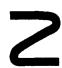
\includegraphics[keepaspectratio]{images/part001_c576909a.jpg}}

\begin{enumerate}
\def\labelenumi{\arabic{enumi}.}
\setcounter{enumi}{5}
\item
  Some passages in the text are designed to forewarn the reader against serious errors. These passages are signposted in the margin with the sign (``dangerous bend'').
\item
  The Exercises are designed both to enable the reader to satisfy himself that he has digested the text and to bring to his attention results that have no place in the text but are nevertheless of interest. The most difficult exercises bear the sign ¶.
\item
  In general, we have adhered to the commonly accepted terminology, except where there appeared to be good reasons for deviating from it.
\item
  We have made a particular effort always to use rigorously correct language, without sacrificing simplicity. As far as possible we have drawn attention in the text to abuses of language, without which any mathematical text runs the risk of pedantry, not to say unreadability.
\item
  Since in principle the text consists of the dogmatic exposition of a theory, it contains in general no references to the literature. Bibliographical references are gathered together in Historical Notes. The bibliography which follows each historical note contains in general only those books and original memoirs that have been of the greatest importance in the evolution of the theory under discussion. It makes no pretense of any sort to completeness.
\end{enumerate}

As to the exercises, we have not thought it worthwhile in general to indicate their origins, since they have been drawn from many different sources (original papers, textbooks, collections of exercises).

\begin{enumerate}
\def\labelenumi{\arabic{enumi}.}
\setcounter{enumi}{10}
\tightlist
\item
  References to a part of this series are given as follows:
\end{enumerate}

\begin{enumerate}
\def\labelenumi{\alph{enumi})}
\item
  If reference is made to theorems, axioms, or definitions presented in the same section (§), they are cited by their number.
\item
  If they occur in another section of the same chapter, this section is also cited in the reference.
\item
  If they occur in another chapter in the same Book, the chapter and section are cited.
\item
  If they occur in another Book, the Book is cited first, by the abbreviation of its title.
\end{enumerate}

The Summaries of Results are cited by the letter R; thus S, R signifies the ``Summary of Results of the Theory of Sets''.

\chapter*{Introduction}
\phantomsection
\addcontentsline{toc}{chapter}{Introduction}

The concept of measure of magnitudes is fundamental, as well in everyday life (length, area, volume, weight) as in experimental science (electric charge, magnetic mass, etc.). The common characteristic of the `measures' of such diverse magnitudes lies in the association of a number to each portion of space fulfilling certain conditions, in such a way that, to the union of two such portions (assumed to be without common point), there corresponds the sum of the numbers assigned to each of them (the additivity of the measure) (*). Moreover, the measure is usually a positive number, and this implies that it is an increasing function of the portion of space measured (**). It will be observed on the other hand that in practice, one hardly ever worries about specifying which portions of space are to be regarded as `measurable'; it is of course indispensable to settle this matter unambiguously in every mathematical theory of measure; for example, this is what one does in elementary geometry when one defines the area of polygons or the volume of polyhedra; in all of these cases, the family of `measurable' sets must naturally be such that the union of any two of them having no point in common is also `measurable'.

In most of the above examples, the measure of a portion of space tends to 0 with its diameter: classically, a point `has no length', which means that it is contained in intervals of arbitrarily small length, consequently one can only assign to it the length 0; the measures of such magnitudes are said to be `diffuse'. However, developments in Mechanics and Physics have introduced the notion of magnitudes for which an object of negligible dimensions may still have non-negligible measure: gravitational or electrical `point masses', which, to tell the truth, are largely mathematical fictions more than they are strictly experimental notions. One is thus led, in Mathematics, to consider measures defined as follows: to each point \(a_i\) ( \(1 \leqslant i \leqslant n\) ) of a finite set \(F\) there is attached a number \(m_i\) , its `mass' or its `weight', and the measure of an arbitrary set \(A\) is the sum of the masses \(m_i\) of the points \(a_i\) that belong to \(A\) .

Closely tied to the concept of measure is that of weighted sum. For example, consider in space a finite number of masses (gravitational or electrical) \(m_{i}\) placed at points \(a_{i}\) (with coordinates \(x_{i}, y_{i}, z_{i}\) ); the component along Oz (for example) of the attraction exerted on a point b (with mass 1 and coordinates \(\alpha, \beta, \gamma\) ) by the set of these masses is (for a suitable system of units) the sum

\[
\sum_ {i} m _ {i} \frac {(z _ {i} - \gamma)}{r _ {i} ^ {3}},
\]

\(r_i^2 = (x_i - \alpha)^2 + (y_i - \beta)^2 + (z_i - \gamma)^2\) being the square of the distance between the points \(a_i\) and \(b\) . In other words, one considers the value of the function

\[
f (x, y, z) = \frac {z - \gamma}{\left((x - \alpha) ^ {2} + (y - \beta) ^ {2} + (z - \gamma) ^ {2}\right) ^ {3 / 2}}
\]

at each point \(a_{i}\) , one multiplies it by the `weight' of this point, and one sums up the `weighted values' of f so obtained. It is known that such sums intervene constantly in Mechanics: centers of gravity and moments of inertia are the best-known examples.

If one wants to extend the notion of `weighted sum' from the case of point masses to that of a `diffuse' measure, where every point has measure zero, one finds oneself in the presence of the problem, of so paradoxical an aspect, that gave rise to the Integral Calculus: how to assign a meaning to a `sum' with infinitely many terms each of which, taken by itself, is zero. Let us take up again the example of calculating the attraction exerted on a point, when the attracting masses are `distributed continuously' throughout a volume V. If V is decomposed into a finite number of (pairwise disjoint) subsets \(V_{i}\) , one assumes that the component along Oz of the attraction exerted by V on a point b is the sum of the components of the attractions exerted on b by each of the \(V_{i}\) . But if the diameter of each \(V_{i}\) is small, the continuous function \(f(x,y,z)\) varies little in \(V_{i}\) , and one is led to liken the attraction exerted by \(V_{i}\) to that which would be exerted by a point mass equal to the mass \(m_{i}\) of \(V_{i}\) and placed at any point \(a_{i}\) of the volume \(V_{i}\) . One is thus led to take, as an approximate value of the sought-for number, the `Riemann sum' \(\sum m_{i}f(x_{i},y_{i},z_{i})\) ; for this to be justified from the mathematical point of view, it must naturally be proved that these approximate values tend to a limit as the maximum diameter of the \(V_{i}\) tends to 0, which is an easy consequence of the uniform continuity of the function f in V (assuming V is compact and the point b is not in V).

It is known that the `method of exhaustion' of the Greeks and `Cavalieri's principle' for the systematic calculation of plane areas and of volumes are based on an analogous procedure, by the decomposition into `slices' of the areas and volumes considered; the `weighted sums' thus arrived at are none other than the integrals \(\int_{a}^{b} f(x) dx\) (cf.~the Historical Note for Chs. I--III of Book IV). Here again, it is the uniform continuity of f that implies the existence of the limit of the `Riemann sums'; more generally, it implies the existence of a limit for the analogous sums \(\sum_{i} f(\xi_{i})(g(x_{i+1}) - g(x_{i}))\)

\((x_{i} \leqslant \xi_{i} \leqslant x_{i+1})\) , where g is only assumed to be a bounded function that is increasing on \([a, b]\) . This limit, denoted \(\int_{a}^{b} f(x) dg(x)\) and called the Stieltjes integral of f with respect to g, may be regarded as the `weighted sum' of the function f for the measure \(\mu\) defined on the set of semi-open intervals \([\alpha, \beta]\) by the formula \(\mu([\alpha, \beta]) = g(\beta+) - g(\alpha+)\) ; it is no longer tied to Differential Calculus as closely as the usual notion of integral (*). The same is true for the classical `double' and `triple' integrals, associated with the measurement of plane areas and volumes, respectively. However, all of these notions of integral are related to each other, not only by their definition, but by the following characteristics: the `integral' \(\mu(f)\) of a continuous numerical function f on a certain compact subset K of the line, the plane, or 3-dimensional space, is a number associated with the element f of the space \(\mathcal{C}(K)\) of continuous functions on K; \(f \mapsto \mu(f)\) is thus a mapping of \(\mathcal{C}(K)\) into R (sometimes called a `functional') that is: \(1^{\circ} linear\) (that is, \(\mu(\alpha f + \beta g) = \alpha \mu(f) + \beta \mu(g)\) for all scalars \(\alpha, \beta\) and continuous functions f, g); \(2^{\circ} positive\) (that is, \(\mu(f) \geqslant 0\) for every continuous function \(f \geqslant 0\) ).

It is remarkable that, conversely, these two properties suffice to characterize the Stieltjes integrals on an interval \([a,b]\) (F. Riesz's theorem). If this is so it is because, starting with the values of the integral of continuous functions, one can reconstitute the measure that gave birth to it. This amounts (if we think of the interpretation of \(\int_{a}^{b}f(x)dx\) as a plane area) to calculating the integral of a characteristic function of an interval, assuming it to be known for continuous functions. In other terms, it is a question of extending in a suitable way the functional \(\mu(f)\) to a set of functions containing \(\mathcal{C}(K)\) and large enough to contain also the characteristic functions of intervals.

There are several methods for accomplishing this extension; one of the most interesting appeals to the notion of function space. One knows that, on the space \(\mathbf{R}^n\) , the norms \(\| \mathbf{x}\|_{\infty} = \sup_{1\leqslant i\leqslant n}|x_i|\) and \(\| \mathbf{x}\|_1 = \sum_{i=1}^{n}|x_i|\) define the same topology. By `passing from finite to infinite' one is led to consider, on the space \(\mathcal{C}(\mathrm{K})\) of continuous functions on a compact interval \(\mathrm{K} = [a,b]\) of \(\mathbf{R}\) , the norms \(\| f\|_{\infty} = \sup_{x\in \mathrm{K}}|f(x)|\) and \(\| f\|_1 = \int_a^b |f(x)|dx\) (or \(\int_a^b |f|dg\) in the case of a Stieltjes integral). But here, the topologies defined by these two norms are different, and the space \(\mathcal{C}(\mathrm{K})\) , which is complete for the first norm (GT, X, §1, No.~6, Cor. 1 of Th. 2), is no longer so for the second. More precisely, one can identify the elements of the completion of \(\mathcal{C}(\mathrm{K})\) for the norm \(\| f\|_1\) with classes of not necessarily continuous functions, and the extension of the integral is then made simply by extending by continuity the functional \(\mu(f)\) defined on \(\mathcal{C}(\mathrm{K})\) , to the completion of this space (the technical details of this procedure are exposed in Ch. IV). Of course, we have assumed that the integral of continuous functions was defined starting with a measure (by the procedure of `Riemann sums' reviewed above); to obtain F. Riesz's theorem, it is necessary to operate in the same way, but by defining the norm to be \(\mu(|f|)\) , where \(\mu(f)\) is the positive linear functional defined on \(\mathcal{C}(\mathrm{K})\) .

The method of extension we have just sketched not only leads to Riesz's theorem, but in addition it permits defining the integral for classes of functions `much more discontinuous' than the characteristic functions of intervals; on considering the characteristic functions of sets that are `integrable' functions, it permits, at the same stroke, extending to the corresponding sets the measure given initially only for intervals, by setting \(\mu(A) = \mu(\varphi_A)\) ; this extension of course preserves the fundamental properties of additivity and positivity of the measure.

The foregoing deals with the Stieltjes integral on the line, but the method of extension carries over at once to measures defined in the plane or in space, or on curves or surfaces. More generally, on analyzing the proofs, one perceives that they are actually valid for every positive linear functional defined on the space \(\mathcal{H}(X)\) of continuous functions on an arbitrary locally compact space X, each of which is zero outside a compact subset (depending on the particular function).

This category of spaces to which the theory of integration is therefore applicable includes naturally the numerical spaces \(R^{n}\) as well as manifolds; it also includes the discrete spaces (where the theory of integration merges with that of summable families of real numbers (GT, IV, §7)), as well as the products (finite or infinite) of compact spaces identical to an interval of R or to a finite set; we shall see later on that the theory of measure on such products plays an important role in the Calculus of Probability.

The extension of the concept of measure to general locally compact spaces has shown itself to be especially fertile in the theory of locally compact groups; generally speaking, the notion of integral appears to be the right tool whenever, in Topological Algebra, one wants to `pass from the finite to the infinite', that is, to generalize the procedures of pure algebra in which finite sums appear, to the case that the `summation' must deal with an infinite number of terms. For example, one knows (A, III, §2) that the elements of the algebra of a finite group G (over the field \(\mathbf{R}\) ) are the mappings \(s \mapsto \alpha(s)\) of G into \(\mathbf{R}\) , with the multiplication law \(\alpha * \beta = \gamma\) , where \(\gamma\) is the function defined by

\[
\gamma (s) = \sum_ {t \in G} \alpha (t) \beta (t ^ {- 1} s).
\]

What appears to be a natural generalization of this algebra, for an arbitrary locally compact group G, is the set of mappings of G into R that are integrable for a certain special measure \(\mu\) on G (the `Haar measure'), the multiplication in the algebra being given by

\[
(f * g) (s) = \int f (t) g (t ^ {- 1} s) d \mu (t).
\]

Moreover, once embarked on this path, one is quickly annoyed by the obligation to `sum' only functions with real values; in many cases, it is useful to know how to define the integral of functions that are defined on X and take values in a topological vector space over R, for example a Banach space or a space of operators on a Banach space. One ascertains that this extension can be made easily with no need for any profound modifications of the theory of integration.

In the foregoing sketch, a preponderant role has been given to continuous functions; it is natural to ask whether the notion of measure is in effect tied in an essential way to the existence of a topology on the set X where it is defined. A close examination of the theory shows that this is not at all the case, and that the methods of extension apply as well to a positive linear functional \(\mu(f)\) defined on a vector space V consisting of numerical functions defined on an arbitrary set X, by means of certain supplementary conditions imposed on V and on \(\mu(f)\) ; these conditions are automatically satisfied when V is a space \(\mathcal{K}(\mathrm{X})\) of continuous functions with compact support, but they are also satisfied in more general cases. However, this greater generality is in some respects illusory: indeed, it can be shown that every `abstract measure' is, in a certain sense, `isomorphic' to a measure defined (starting with continuous functions) on a suitable locally compact space; on the other hand, most applications have to do with sets X equipped with a topology that intervenes naturally in the matter; we shall therefore occupy ourselves exclusively, until Chapter IX, with measures defined on locally compact spaces.

The first two chapters are preliminaries to the theory: they are devoted to the proof of inequalities fundamental to the extension, and to the study of certain ordered vector spaces, the Riesz spaces, which play an important role in several questions later on.

The concept of measure on a locally compact space is defined in Chapter III; we take as point of departure the theorem of Riesz, which thus becomes a definition: the integral of continuous functions is therefore defined before the measure of sets, as a positive linear functional on \(\mathcal{K}(\mathrm{X})\) . This presentation offers certain technical advantages (due notably to the fact that the continuous functions form a vector space, whereas this is not the case for the characteristic functions of sets); moreover, it is in the form of a functional on \(\mathcal{K}(\mathrm{X})\) that the integral naturally arises in numerous questions. Finally, the differences of two positive linear functionals on \(\mathcal{K}(\mathrm{X})\) (which we again call measures on X) may be characterized as the linear forms on \(\mathcal{K}(\mathrm{X})\) satisfying certain continuity conditions; the theory of integration is thus related, on the one hand to the general theory of duality in topological vector spaces (cf.~Book V) and on the other hand to the theory of distributions, which generalize certain aspects of the concept of measure and which we shall expose in a later Book.

Chapter IV is devoted to the extension of the integral; both integrable functions and the measure of sets are defined there, as well as the function spaces \(L^{p}\) , whose importance in applications is considerable; also shown there, is how the introduction of the concept of measurable function leads to convenient criteria for integrability.

In the next two chapters, it will be seen how measurable functions appear also as `densities', enabling one to define new measures on a space X starting from a given measure. This study, which leads in particular to important results in the duality theory of the \(L^{p}\) spaces, is also tied to the notion of vectorial measure, which can, in the most favorable cases, be brought under the theory of integration (with respect to a positive measure) of vector-valued functions.

We shall also develop what may be considered the modern culmination of the idea of `decomposition into slices' of plane areas and of volumes, introduced by the founders of the Integral Calculus: under certain conditions, a measure on a space X can be decomposed into a `sum' of measures each of which is carried by a `slice' of the space X (that is, by an equivalence class with respect to a certain relation R); moreover, such a decomposition permits calculating the integral of a function, with respect to the original measure, by first integrating `over each slice', then integrating (with respect to a suitable measure) the resulting function on the quotient space X/R (a generalization of `double summation' for the sum of a family where the indices run over a product set).

Chapter VII is devoted to the study of Haar measure on a locally compact group, which is characterized, up to a scalar multiple, by the property of being invariant under every left translation of the group.

In Chapter VIII the convolution of measures is exposed, a concept that plays a role of the first order in modern Functional Analysis.

Chapter IX is devoted to integration in Hausdorff topological spaces that are not necessarily locally compact, and in particular in locally convex vector spaces; this permits, notably, the extension of the theory of the Fourier transformation to the latter spaces. The mode of exposition chosen in the early sections consists in reducing, to the extent possible, to the case of compact spaces treated in the earlier chapters.

\chapter{Inequalities of convexity}

\section{The fundamental inequality of convexity}

Let X be a set; in the vector space \(R^{X}\) of all finite numerical functions \(^{1}\) defined on X, let P be the set of all positive real-valued functions on X. On the other hand, let M be a numerical function, \(^{2}\) finite or not, with values \(\geqslant0\) , defined on P, such that:

\(1^{\circ} M(0) = 0\) , and \(M\) is positively homogeneous, that is, \(M(\lambda f) = \lambda M(f)\) for every real number \(\lambda > 0\) .

\(2^{\circ} M\) is increasing in P, in other words the relation \(f \leqslant g\) implies \(M(f) \leqslant M(g)\) .

\(3^{\circ} M\) is convex in P, in other words (TVS, II, §2, No.~8) satisfies the relation \(M(f + g) \leqslant M(f) + M(g)\) .

Example. --- Suppose X is a finite set, for example the interval \([1,n]\) of N; denoting by \(x_{i}\) ( \(1 \leqslant i \leqslant n\) ) the coordinates of a vector \(x \in R^{n}\) , the functions \(M_{1}(\mathbf{x}) = \sum_{i=1}^{n} x_{i}\) and \(M_{\infty}(\mathbf{x}) = \sup_{1 \leqslant i \leqslant n} x_{i}\) satisfy the preceding conditions in the set P of vectors x with coordinates \(\geqslant 0\) .

Remark. --- Let S be a pointed convex cone contained in P (that is, a set such that \(S + S \subset S\) and \(\lambda S \subset S\) for \(\lambda \geqslant 0\) ; cf.~TVS, II, §2, No.~4); let M be a numerical function (finite or not) with values \(\geqslant 0\) , defined on S and satisfying in S the above conditions \(1^{\circ}\) , \(2^{\circ}\) and \(3^{\circ}\) . Then M can be extended to the entire set P, in such a way that the extended function (which we denote again by M) satisfies the same conditions: it suffices, for every function \(f \in P\) , to set \(M(f) = +\infty\) if there does not exist any function \(g \in S\) such that \(f \leqslant g\) , and \(M(f) = \inf_{g \in S, f \leqslant g} M(g)\) in

the contrary case. This procedure will be applied in Ch. IV, §1 to define the upper integral of a positive function.

PROPOSITION 1. --- Let \(\varphi(t_{1}, t_{2}, \ldots, t_{n})\) be a finite numerical function, defined and continuous for \(t_{i} \geqslant 0\) ( \(1 \leqslant i \leqslant n\) ), such that:

\(1^{\circ}\) the relations \(t_i > 0\) \((1\leqslant i\leqslant n)\) imply \(\varphi (t_1,t_2,\dots ,t_n) > 0\)

\(2^{\circ}\) the function \(\varphi\) is positively homogeneous;

\(3^{\circ}\) the set \(\mathbf{K} \subset \mathbf{R}^{n}\) defined by the relations \(t_{i} \geqslant 0\) ( \(1 \leqslant i \leqslant n\) ) \(\varphi(t_{1}, t_{2}, \ldots, t_{n}) \geqslant 1\) is convex.

Under these conditions, if \(f_1, f_2, \ldots, f_n\) are \(n\) finite functions \(\geqslant 0\) defined on \(X\) , such that \(M(f_i) < +\infty\) for \(1 \leqslant i \leqslant n\) , then

\[
M \left(\varphi \left(f _ {1}, f _ {2}, \dots , f _ {n}\right)\right) \leqslant \varphi \left(M \left(f _ {1}\right), M \left(f _ {2}\right), \dots , M \left(f _ {n}\right)\right).\tag{1}
\]

One knows, by the Hahn-Banach theorem (TVS, II, §5), that K is the intersection of the n half-spaces \(t_{i} \geqslant 0\) ( \(1 \leqslant i \leqslant n\) ) and a family of closed half-spaces \((\mathrm{U}_{\iota})_{\iota \in \mathrm{I}}\) , \(U_{\iota}\) being defined by a relation of the form

\[
\alpha_ {\iota 1} t _ {1} + \alpha_ {\iota 2} t _ {2} + \dots + \alpha_ {\iota n} t _ {n} - \beta_ {\iota} \geqslant 0,\tag{2}
\]

where the \(\alpha_{\iota k}\) are not all zero. By hypothesis, if \(\mathbf{t}=(t_{i})\) is such that \(t_{i}>0\) for \(1\leqslant i\leqslant n\) , then \(\varphi(t_{1},\ldots,t_{n})>0\) , therefore there exists a \(\lambda_{0}>0\) such that the relation \(\lambda\geqslant\lambda_{0}\) implies \(\lambda t\in K\) ; this shows that, for each \(\iota\in I\) , the relations \(t_{i}\geqslant0\) ( \(1\leqslant i\leqslant n\) ) imply \(\alpha_{\iota1}t_{1}+\cdots+\alpha_{\iota n}t_{n}\geqslant0\) and therefore \(\alpha_{\iota k}\geqslant0\) for \(1\leqslant k\leqslant n\) ; it is then clear that K is also the intersection of the half-spaces \(t_{i}\geqslant0\) ( \(1\leqslant i\leqslant n\) ) and the \(U_{\iota}\) such that \(\beta_{\iota}\geqslant0\) ; moreover, since the origin does not belong to K, there exists at least one index \(\iota\) such that \(\beta_{\iota}>0\) .

Now let C be the convex cone in \(R^{n+1}\) defined by the relations \(t_{i} \geqslant 0\) ( \(1 \leqslant i \leqslant n + 1\) ), \(t_{n+1} \leqslant \varphi(t_{1}, t_{2}, \ldots, t_{n})\) (the closure of the convex cone generated in \(R^{n+1}\) by the convex set \(K \times \{1\}\) ); it is immediate that C is also defined by the relations \(t_{i} \geqslant 0\) ( \(1 \leqslant i \leqslant n + 1\) ) and

\[
\beta_ {\iota} t _ {n + 1} \leqslant \alpha_ {\iota 1} t _ {1} + \dots + \alpha_ {\iota n} t _ {n} \quad (\iota \in \mathrm{I}, \beta_ {\iota} \geqslant 0).\tag{3}
\]

For every \(x \in X\) , we therefore have

\[
\beta_ {\iota} \varphi (f _ {1} (x), \dots , f _ {n} (x)) \leqslant \alpha_ {\iota 1} f _ {1} (x) + \dots + \alpha_ {\iota n} f _ {n} (x)\tag{4}
\]

for all \(\iota \in I\) . For every index \(\iota\) such that \(\beta_{\iota} > 0\) , it follows from (4) and the hypotheses on \(M\) that \(M(\varphi(f_1, f_2, \ldots, f_n))\) is finite and

\[
\beta_ {\iota} M \left(\varphi \left(f _ {1}, f _ {2}, \dots , f _ {n}\right)\right) \leqslant \alpha_ {\iota 1} M \left(f _ {1}\right) + \alpha_ {\iota 2} M \left(f _ {2}\right) + \dots + \alpha_ {\iota n} M \left(f _ {n}\right),
\]

and this relation is also verified in an obvious manner if \(\beta_{\iota} = 0\) . We thus

see that the point with coordinates

\[
M (f _ {1}), M (f _ {2}), \dots , M (f _ {n}), M (\varphi (f _ {1}, f _ {2}, \dots , f _ {n}))
\]

belongs to C, which proves the proposition.

\section{The inequalities of Hölder and Minkowski}

In this No.~and in the following one, X and P have the same meaning as in No.~1, and M denotes a function defined on P that satisfies the conditions listed in No.~1.

PROPOSITION 2. --- Let \(\alpha\) and \(\beta\) be two numbers such that \(0 < \alpha < 1\) , \(0 < \beta < 1\) , \(\alpha + \beta = 1\) . If \(f\) and \(g\) are two finite functions \(\geqslant 0\) defined on X, and if \(M(f)\) and \(M(g)\) are finite, then

\[
M (f ^ {\alpha} g ^ {\beta}) \leqslant (M (f)) ^ {\alpha} (M (g)) ^ {\beta}\tag{5}
\]

(Hölder's inequality).

By Prop. 1, it all comes down to proving that, in \(\mathbf{R}^2\) , the set defined by the relations \(t_1 \geqslant 0\) , \(t_2 \geqslant 0\) , \(t_1^\alpha t_2^\beta \geqslant 1\) is convex, or again (FRV, I, §4, No.~1, Def. 1) that the function \(u(t) = t^{-\alpha/\beta}\) is convex for \(0 < t < +\infty\) . Now, setting \(r = \alpha/\beta\) , we have \(\mathrm{D}^2 u(t) = r(r + 1)t^{-r - 2}\) and, since \(r > 0\) , \(\mathrm{D}^2 u(t) > 0\) on \(]0, +\infty[\) , which proves the proposition (FRV, I, §4, No.~4, Cor. of Prop. 8).

COROLLARY. --- Let \(\alpha_{i}\) ( \(1 \leqslant i \leqslant n\) ) be n numbers \(\geqslant 0\) such that \(\sum_{i=1}^{n} \alpha_{i} = 1\) , and let \(f_{i}\) ( \(1 \leqslant i \leqslant n\) ) be n functions \(\geqslant 0\) defined on X, such that \(M(f_{i})\) is finite for \(1 \leqslant i \leqslant n\) . Under these conditions,

\[
M \left(f _ {1} ^ {\alpha_ {1}} f _ {2} ^ {\alpha_ {2}} \dots f _ {n} ^ {\alpha_ {n}}\right) \leqslant \left(M (f _ {1})\right) ^ {\alpha_ {1}} \left(M (f _ {2})\right) ^ {\alpha_ {2}} \dots \left(M (f _ {n})\right) ^ {\alpha_ {n}}.\tag{6}
\]

We can restrict attention to the case that \(\alpha_{i} > 0\) for every i. It suffices to argue by induction on n, by applying the inequality (5) to the numbers \(\alpha = \alpha_{1}\) and \(\beta = \sum_{i=2}^{n} \alpha_{i}\) , and to the functions \(f = f_{1}\) , \(g = (f_{2}^{\alpha_{2}} f_{3}^{\alpha_{3}} \cdots f_{n}^{\alpha_{n}})^{1/\beta}\) .

PROPOSITION 3. --- Let p be a real number \(\geqslant 1\) . If f and g are two finite functions \(\geqslant 0\) defined on X, then

\[
\left(M \big ((f + g) ^ {p} \big)\right) ^ {1 / p} \leqslant \left(M (f ^ {p})\right) ^ {1 / p} + \left(M (g ^ {p})\right) ^ {1 / p}\tag{7}
\]

(Minkowski's inequality).

We can restrict attention to the case that \(M(f^{p})\) and \(M(g^{p})\) are finite. By Prop. 1, we are reduced to proving that the set in \(R^{2}\) defined by the relations \(t_{1} \geqslant 0\) , \(t_{2} \geqslant 0\) , \(t_{1}^{1/p} + t_{2}^{1/p} \geqslant 1\) is convex, or again that the function \(u(t) = (1 - t^{1/p})^{p}\) is convex for \(0 \leqslant t \leqslant 1\) . Now,

\[
\mathrm{D} ^ {2} u (t) = \left(1 - \frac {1}{p}\right) t ^ {1 / p - 2} (1 - t ^ {1 / p}) ^ {p - 2} \geqslant 0
\]

for \(0 < t \leqslant 1\) , whence the proposition.

\section{\texorpdfstring{The semi-norms \(\mathbf{N}_p\)}{The semi-norms N sub p}}

Let \(p\) be a real number \(\geqslant 1\) and let \(\mathcal{F}^p(\mathrm{X},M)\) be the set of finite numerical functions \(f\) defined on \(\mathrm{X}\) such that \(M(|f|^p)\) is finite. It is obvious that if \(g\) is a function belonging to \(\mathcal{F}^p(\mathrm{X},M)\) and if \(|f| \leqslant |g|\) , then \(f\) also belongs to \(\mathcal{F}^p(\mathrm{X},M)\) ; this remark and Minkowski's inequality show that the sum of two functions in \(\mathcal{F}^p(\mathrm{X},M)\) also belongs to this set; taking into account the fact that \(M\) is positively homogeneous, we thus see that \(\mathcal{F}^p(\mathrm{X},M)\) is a linear subspace of the space \(\mathbf{R}^{\mathrm{X}}\) of all finite numerical functions defined on \(\mathrm{X}\) .

For every number \(p > 0\) and every finite numerical function \(f\) defined on \(X\) , set

\[
\mathrm{N} _ {p} (f) = \left(M (| f | ^ {p})\right) ^ {1 / p};
\]

then \(\mathrm{N}_p(\lambda f) = |\lambda |\mathrm{N}_p(f)\) for every scalar \(\lambda\) ; moreover, if \(p \geqslant 1\) then, by (7),

\[
\mathrm{N} _ {p} (f + g) \leqslant \mathrm{N} _ {p} (f) + \mathrm{N} _ {p} (g),\tag{8}
\]

which proves that \(N_{p}\) is a semi-norm on the vector space \(\mathcal{F}^{p}(X,M)\) (TVS, II, §1).

PROPOSITION 4. --- Let p and q be two real numbers \textgreater{} 0 and set \(1/r = 1/p + 1/q\) . For any finite numerical functions f, g defined on X,

\[
\mathrm{N} _ {r} (f g) \leqslant \mathrm{N} _ {p} (f) \mathrm{N} _ {q} (g)\tag{9}
\]

provided that \(\mathrm{N}_p(f)\) and \(\mathrm{N}_q(g)\) are finite.

For, the relation (9) may be written

\[
M (| f | ^ {r} | g | ^ {r}) \leqslant \bigl (M (| f | ^ {p}) \bigr) ^ {r / p} \bigl (M (| g | ^ {q}) \bigr) ^ {r / q},
\]

which is none other than Hölder's inequality (5) applied to the numbers \(\alpha = r / p\) and \(\beta = r / q\) and to the functions \(|f|^p\) and \(|g|^q\) .

COROLLARY. --- Suppose that \(M(1) = 1\) ; then, for every finite numerical function f defined on X, the mapping \(p \mapsto \mathrm{N}_{p}(f)\) is increasing in {]}0, +∞{[}.

Applying the inequality (9) to the case that g = 1, we see that \(\mathrm{N}_{r}(f) \leqslant \mathrm{N}_{p}(f)\) for all q \textgreater{} 0; since the number r defined by \(1/r = 1/p + 1/q\) runs over the set of numbers such that 0 < r < p when q runs over the set of numbers \textgreater{} 0, the corollary is proved.

PROPOSITION 5. --- For every finite numerical function f defined on X, the set I of values of 1/p (p \textgreater{} 0) such that \(\mathrm{N}_{p}(f)\) is finite is either empty or is an interval; if I is not reduced to a point, then the mapping \(\alpha \mapsto \log \mathrm{N}_{1/\alpha}(f)\) is either convex on I or is equal to \(-\infty\) on the interior of I.

Let r and s be two distinct numbers \textgreater{} 0 such that 1/r and 1/s belong to I; it all comes down to proving that if

\[
{\frac {1}{p}} = {\frac {t}{r}} + {\frac {1 - t}{s}},
\]

with \(0 < t < 1\) , then

\[
\log \mathrm{N} _ {p} (f) \leqslant t \cdot \log \mathrm{N} _ {r} (f) + (1 - t) \log \mathrm{N} _ {s} (f),\tag{10}
\]

or, what comes to the same,

\[
\mathrm{N} _ {p} (f) \leqslant \left(\mathrm{N} _ {r} (f)\right) ^ {t} \left(\mathrm{N} _ {s} (f)\right) ^ {1 - t},\tag{11}
\]

a relation that may, by the definition of \(N_{p}\) , be written

\[
M (| f | ^ {p}) \leqslant \left(M (| f | ^ {r})\right) ^ {t p / r} \left(M (| f | ^ {s})\right) ^ {(1 - t) p / s}.\tag{12}
\]

Setting \(\alpha = tp / r\) , we have \(1 - \alpha = (1 - t)p / s\) by the relation that defines \(p\) as a function of \(t, r, s\) ; whence \(p = \alpha r + (1 - \alpha)s\) . Hölder's inequality now yields

\[
M \big (| f | ^ {r \alpha} | f | ^ {s (1 - \alpha)} \big) \leqslant \big (M (| f | ^ {r}) \big) ^ {\alpha} \big (M (| f | ^ {s}) \big) ^ {1 - \alpha},
\]

which is none other than the inequality (12).

\chapter*{Exercises}
\phantomsection
\addcontentsline{toc}{chapter}{Exercises}

\begin{enumerate}
\def\labelenumi{\arabic{enumi})}
\item
  With the hypotheses of No.~1, show that the set of bounded functions on X such that \(M(|f|)\) is finite is a subalgebra A of \(\mathbf{R}^X\) , and that the set of bounded functions on X such that \(M(|f|) = 0\) is an ideal in A. If, moreover, \(M(1)\) is finite, show that the mapping \(f \mapsto M(f)\) is continuous when A is equipped with the topology of uniform convergence in X.
\item
  Let X be the interval \([0, +\infty[\) of R, S the convex cone formed by the functions defined on X such that \(0 \leqslant f(x) \leqslant kx\) on X (for a finite number k \textgreater{} 0 depending on f). Set \(M(f) = 0\) for \(f \in S\) , and \(M(f) = +\infty\) for every positive function f defined on X and not belonging to S. Show that M satisfies the conditions of No.~1, and that \(M(x) = 0\) , and \(M(x^{r}) = +\infty\) for every number r \textgreater{} 0 not equal to 1.
\item
  Give an example where \(X\) is a set with two elements, \(N sub p(\mathbf{x})\) is finite for every \(p > 0\) and every \(\mathbf{x} \in \mathbf{R}^2\) , but where there exist values of \(p\) such that the mapping \(p \mapsto N sub p(\mathbf{x})\) is not differentiable at these points.
\item
  Deduce the inequality (6) from the inequality of the geometric mean
\end{enumerate}

\[
z _ {1} ^ {\alpha_ {1}} z _ {2} ^ {\alpha_ {2}} \dots z _ {n} ^ {\alpha_ {n}} \leqslant \alpha_ {1} z _ {1} + \dots + \alpha_ {n} z _ {n} \quad (\text {where} \sum_ {i = 1} ^ {n} \alpha_ {i} = 1)
\]

(FRV, III, §1, No.~1, Prop. 2). (Reduce to the case that \(M(f_i) = 1\) for \(1 \leqslant i \leqslant n\) .)

\begin{enumerate}
\def\labelenumi{\arabic{enumi})}
\setcounter{enumi}{4}
\tightlist
\item
  Let \(\alpha\) be a real number \(>1\) and let \(\beta = 1 - \alpha < 0\) . Let \(g\) be a finite function, defined on X, such that \(g(x) > 0\) for all \(x \in X\) and such that \(M(g) > 0\) ; show that for every finite function \(f \geqslant 0\) defined on X such that \(M(f)\) is finite,
\end{enumerate}

\[
M (f ^ {\alpha} g ^ {\beta}) \geqslant (M (f)) ^ {\alpha} (M (g)) ^ {\beta}
\]

(apply Hölder's inequality suitably).

\begin{enumerate}
\def\labelenumi{\arabic{enumi})}
\setcounter{enumi}{5}
\tightlist
\item
  Deduce Minkowski's inequality from Hölder's inequality (find an upper bound for \(M(f(f + g)^{p-1})\) with the help of Hölder's inequality). If one assumes that \(M(f + g) = M(f) + M(g)\) for every pair of functions \(f, g\) defined and \(\geqslant 0\) on \(X\) , deduce similarly from Exer. 5 the inequality
\end{enumerate}

\[
\left(M \big ((f + g) ^ {p} \big)\right) ^ {1 / p} \geqslant \left(M (f ^ {p})\right) ^ {1 / p} + \left(M (g ^ {p})\right) ^ {1 / p}
\]

in the following cases:

\begin{enumerate}
\def\labelenumi{\alph{enumi})}
\tightlist
\item
  \(0 < p < 1\) , \(f\) and \(g\) finite functions \(\geqslant 0\) defined on X, such that \(f(x) + g(x) > 0\) for all \(x \in X\) and such that \(M(f^p)\) and \(M(g^p)\) are finite; b) \(p < 0\) , \(f\) and \(g\) finite functions defined on X, such that \(f(x) > 0\) and \(g(x) > 0\) for all \(x \in X\) , \(M(f^p)\) and \(M(g^p)\) are finite, and \(M((f + g)^p) > 0\) .
\end{enumerate}

\chapter*{HISTORICAL NOTE}
\phantomsection
\addcontentsline{toc}{chapter}{HISTORICAL NOTE}

(N.B. --- The Roman numerals refer to the bibliography at the end of this note.)

The concepts of arithmetic mean and geometric mean of two positive quantities go back to antiquity, in particular the Pythagoreans made of them one of their favorite subjects. It is also probable that the inequality \(\sqrt{ab} \leqslant \frac{1}{2}(a + b)\) between these means was well-known to them; in any case it is proved by Euclid, in connection with the problem of maximizing the product of two numbers whose sum is given. Apparently one must wait until the rather late date of 1729 to find explicit mention, by MacLaurin, of the generalization of this problem to n numbers, and the corresponding inequality (and this, even though much more difficult extremum problems had been addressed long before).

Other analogous inequalities appeared in Analysis and Geometry from the end of the 18th century onward. Thus, in 1789, Lhuilier solved a geometric maximum problem associated with the inequality

\[
\sqrt {\left(\sum_ {k = 1} ^ {n} a _ {k}\right) ^ {2} + \left(\sum_ {k = 1} ^ {n} b _ {k}\right) ^ {2}} \leqslant \sum_ {k = 1} ^ {n} \sqrt {a _ {k} ^ {2} + b _ {k} ^ {2}};
\]

Cauchy, in 1821, proved the special case

\[
\left(\sum_ {k = 1} ^ {n} a _ {k} b _ {k}\right) ^ {2} \leqslant \left(\sum_ {k = 1} ^ {n} a _ {k} ^ {2}\right) \left(\sum_ {k = 1} ^ {n} b _ {k} ^ {2}\right)
\]

of Hölder's inequality; Buniakowsky in 1859 and H. A. Schwarz in 1885 generalized Cauchy's inequality to integrals.

Nevertheless, it was not until nearly the end of the 19th century that the inequalities of convexity became the object of systematic study. O. Hölder, in 1888 (I), had the idea of introducing convex functions of a single variable into the question: he thus obtained the inequality of the geometric mean starting with the concavity of \(\log x\) ; applying the same idea to the function \(x^{r}\) , he proved the inequality that bears his name, and which had already been found a year earlier by L. J. Rogers starting from the inequality of the geometric mean (cf.~Exer. 4). As for Minkowski's inequality, it was proved by the latter in 1896 (for finite sums), in connection with his memorable works on the `Geometry of numbers' ((II), pp.~115-117); however, while the idea of convexity (for functions of any number of variables) is one of the fundamental concepts of this work, it is rather surprising that Minkowski did not notice that his inequality may be obtained by Hölder's method applied to \((1 + x^{r})^{1 / r}\) (he limited himself to applying the classical methods for seeking an extremum by means of the infinitesimal calculus).

For a deeper study of the inequalities of convexity and of their applications, the reader may consult the book of Hardy, Littlewood and Pólya devoted to the question, which also contains a very complete bibliography (III).

\begin{enumerate}
\def\labelenumi{(\Roman{enumi})}
\item
  O. HÖLDER, Ueber einen Mittelwertsatz, Göttinger Nachrichten (1889), pp.~38-47.
\item
  H. MINKOWSKI, Geometrie der Zahlen, 2nd. edn., Leipzig--Berlin (Teubner), 1910.
\item
  G. H. HARDY, J. E. LITTLEWOOD, G. PÓLYA, Inequalities, Cambridge (University Press), 1934.
\end{enumerate}

\chapter{Riesz spaces}

\section{RIESZ SPACES AND FULLY LATTICE-ORDERED SPACES}

\subsection{Definition of Riesz spaces}

Recall that, on a set E, a vector space structure over the field R and an order structure are said to be compatible if they satisfy the following two axioms:

\((\mathrm{OVS}_{\mathrm{I}})\) The relation \(x \leqslant y\) implies \(x + z \leqslant y + z\) for all \(z \in \mathbb{E}\) .

\((\mathrm{OVS}_{\mathrm{II}})\) The relation \(x \geqslant 0\) implies \(\lambda x \geqslant 0\) for every scalar \(\lambda > 0\) .

The space E, equipped with these two structures, is called an ordered vector space (TVS, II, §2, No.~5).

Axiom (OVS \(_{I}\) ) signifies that the order structure and the additive group structure on E are compatible, in other words that E, equipped with these two structures, is an ordered group (A, VI, §1, No.~1).

Axiom (OVS \(_{\text{I}}\) ) implies that the relations \(x \leqslant y\) and \(x + z \leqslant y + z\) are equivalent. Similarly, it follows from (OVS \(_{\text{II}}\) ) that, for every scalar \(\lambda > 0\) , the relations \(x \leqslant y\) and \(\lambda x \leqslant \lambda y\) are equivalent, because \(\lambda^{-1} > 0\) and so the relation \(\lambda x \leqslant \lambda y\) implies \(\lambda^{-1}(\lambda x) \leqslant \lambda^{-1}(\lambda y)\) . One can therefore say that, in an ordered vector space, the translations and the homotheties of ratio \(> 0\) are automorphisms of the order structure; this fact is also expressed by saying that the order is invariant under every translation and every homothety of ratio \(> 0\) . Moreover, the symmetry \(x \mapsto -x\) is an isomorphism of the order structure of E onto the opposite order structure.

DEFINITION 1. --- An ordered vector space is said to be a Riesz space (or lattice-ordered vector space) \(^{1}\) if its order structure is a lattice-ordering (that is, if every pair of elements x, y of E has a supremum \(\sup(x,y)\) and an infimum \(\inf(x,y)\) ). \(^{2}\)

Example. The space \(\mathbf{R}^{\mathrm{A}}\) of all real-valued functions defined on any set A is a Riesz space (for the order relation \(\ll x(t) \leqslant y(t)\) for all \(t \in \mathrm{A} \gg\) ); for, any two real-valued functions \(x, y\) defined on A have a supremum (resp. an infimum) equal to the mapping \(t \mapsto \sup(x(t), y(t))\) (resp. \(t \mapsto \inf(x(t), y(t))\) ).

One can also say that a Riesz space is a vector space E equipped with an order structure such that, on the one hand, this structure and the additive group structure of E define a lattice-ordered group structure on E (A, VI, §1, No.~9), and on the other hand that the axiom (OVS \(_{II}\) ) is satisfied.

Thus, all of the properties of lattice-ordered groups are applicable to Riesz spaces; we shall review here the principal ones (cf.~A, VI, §1, Nos. 9 to 12), as well as indicating the consequences that flow from the axiom (OVS \(_{II}\) ).

We recall first that one writes \(x^{+} = \sup(x,0)\) (the positive part of x), \(x^{-} = (-x)^{+} = \sup(-x,0)\) (the negative part of x), \(|x| = \sup(x,-x)\) (the absolute value of x); then \(x = x^{+} - x^{-}\) and \(|x| = x^{+} + x^{-}\) ; here, these two relations are equivalent to

\[
x ^ {+} = \frac {1}{2} (| x | + x), \quad x ^ {-} = \frac {1}{2} (| x | - x).
\]

The relation \(x \leqslant y\) is equivalent to \(\ll x^{+} \leqslant y^{+}\) and \(x^{-} \geqslant y^{-}\) . For any \(x\) and \(y\) , the triangle inequality holds:

\[
\vert x + y \vert \leqslant \vert x \vert + \vert y \vert .\tag{1}
\]

By the invariance of order under every homothety of ratio \textgreater{} 0,

\[
\sup (\lambda x, \lambda y) = \lambda \sup (x, y) \quad \text { for   all } \lambda \geqslant 0.\tag{2}
\]

In particular,

\[
(\lambda x) ^ {+} = \lambda x ^ {+}, (\lambda x) ^ {-} = \lambda x ^ {-} \quad \text { for   all } \lambda \geqslant 0.\tag{3}
\]

On the other hand, for \(\lambda < 0\) we have \((\lambda x)^{+} = (-\lambda x)^{-} = |\lambda |x^{-}\) and \((\lambda x)^{-} = (-\lambda x)^{+} = |\lambda |x^{+}\) ; it follows that, for every \(\lambda \in \mathbf{R}\) and every \(x\in \mathrm{E}\) ,

\[
\left| \lambda x \right| = \left| \lambda \right| \cdot \left| x \right|.\tag{4}
\]

The invariance of order under translation shows that for all \(z \in E\) ,

\[
\sup (x + z, y + z) = z + \sup (x, y),\tag{5}
\]

whence, in particular,

\[
\sup (x, y) = x + (y - x) ^ {+} = \frac {1}{2} (x + y + | x - y |).\tag{6}
\]

We have the relations

\[
\inf (x, y) = - \sup (- x, - y),\tag{7}
\]

\[
\sup (x, y) + \inf (x, y) = x + y.\tag{8}
\]

If \(x, y, z\) are \(\geqslant 0\) then (A, VI, §1, No.~12, Prop. 11)

\[
\inf (x + y, z) \leqslant \inf (x, z) + \inf (y, z).\tag{9}
\]

If A and B are two subsets of E each of which has a supremum, then \(A + B\) also has a supremum and

\[
\sup (A + B) = \sup A + \sup B.\tag{10}
\]

Two elements \(x, y\) of \(\mathrm{E}\) are said to be alien \(^3\) (to each other) if \(\inf(|x|, |y|) = 0\) ; by (8), this relation is equivalent to \(\sup(|x|, |y|) = |x| + |y|\) , and also, by (6), to \(||x| - |y|| = |x| + |y|\) ; 0 is the only element alien to itself; for every \(x \in \mathrm{E}\) , \(x^+\) and \(x^-\) are alien and may be characterized as the only alien elements \(y \geqslant 0\) , \(z \geqslant 0\) such that \(x = y - z\) . If \(y\) is alien to \(x\) , then every \(z \in \mathrm{E}\) such that \(|z| \leqslant |y|\) is also alien to \(x\) . If \(y\) and \(z\) are alien to \(x\) , then so is \(|y| + |z|\) , by the inequality (9); in particular, \(n|y|\) is alien to \(x\) for every integer \(n > 0\) , from which it follows that \(\lambda y\) is alien to \(x\) for every scalar \(\lambda\) , since there exists an integer \(n\) such that \(|\lambda| \leqslant n\) , whence \(|\lambda y| \leqslant n|y|\) . If a subset \(A\) of \(E\) consists of elements alien to \(x\) and if \(A\) has a supremum, then that supremum is also alien to \(x\) (A, VI, §1, No.~12, Cor. of Prop. 13).

Finally, we have the decomposition lemma (A, VI, §1, No.~10, Th. 1):

If \((x_{i})_{i\in \mathrm{I}}\), \((y_{j})_{j\in \mathrm{J}}\) are two finite sequences of elements \(\geqslant 0\) of E such that \(\sum_{i\in \mathrm{I}}x_i = \sum_{j\in \mathrm{J}}y_j\) , then there exists a finite sequence \((z_{ij})_{(i,j)\in \mathrm{I}\times \mathrm{J}}\) of elements \(\geqslant 0\) of E such that \(x_{i} = \sum_{j\in \mathrm{J}}z_{ij}\) for all \(i\in \mathrm{I}\) , and \(y_{j} = \sum_{i\in \mathrm{I}}z_{ij}\) for all \(j\in \mathrm{J}\) .

\subsection{Generation of a Riesz space by its positive elements}

Let \(\mathbf{E}\) be an ordered vector space; the set \(\mathrm{P}\) of elements \(\geqslant 0\) of \(\mathbf{E}\) is a convex cone with vertex 0, that is (TVS, II, §2, No.~4), a set such that

\(P + P \subset P\) and \(\lambda P \subset P\) for all \(\lambda > 0\) . Conversely, if, in a vector space E over R, P is a convex cone with vertex 0, such that \(P \cap (-P) = \{0\}\) (in other words, a pointed and proper convex cone), one knows (loc. cit.) that the relation \(y - x \in P\) is an order relation (denoted \(x \leqslant y\) ) compatible with the vector space structure of E. For this order structure to define a Riesz space structure on E, it is necessary and sufficient that:

\(1^{\circ}\) P generates E, that is, every \(z \in \mathbf{E}\) is of the form \(y - x\) , where \(x\) and \(y\) belong to P;

\(2^{\circ}\) P satisfies one of the following two conditions:

\begin{enumerate}
\def\labelenumi{\alph{enumi})}
\item
  every pair of elements of \(\mathbf{P}\) has a supremum in \(\mathbf{P}\) ;
\item
  every pair of elements of P has an infimum in P (A, VI, §1, No.~9, Prop. 8).
\end{enumerate}

\subsection{Fully lattice-ordered spaces}

DEFINITION 2. --- A Riesz space E is said to be fully lattice-ordered if every nonempty subset of E that is bounded above has a supremum in E.

It is immediate that in a fully lattice-ordered space E, every nonempty subset that is bounded below has an infimum in E.

Examples. --- 1) If A is any set, the space \(R^{A}\) of real-valued functions defined on A is fully lattice-ordered, the supremum in \(R^{A}\) of a family that is bounded above being its upper envelope (GT, IV, §5, No.~5).

\begin{enumerate}
\def\labelenumi{\arabic{enumi})}
\setcounter{enumi}{1}
\tightlist
\item
  Let F be any set; the space \(\mathcal{B}(\mathrm{F})\) of bounded real-valued functions on F, equipped with the order structure induced by that of \(R^{F}\) , is fully lattice-ordered. However, if F is a topological space, the space \(\mathcal{C}(\mathrm{F})\) of continuous real-valued functions on F (equipped with the order structure induced by that of \(R^{F}\) ) is a Riesz space that is not in general fully lattice-ordered (cf.~Exer. 13). Consider for example the case that \(F = R\) ; let I be the interval {]}0,1{[}, \(\varphi_{I}\) the characteristic function of I, and let H be the set of continuous functions \(x(t)\) such that \(x \leqslant \varphi_{I}\) ; it is clear that H is bounded above in \(\mathcal{C}(\mathrm{F})\) . The function \(\varphi_{I}\) is the upper envelope of the \(x \in H\) , but it is not their supremum in \(\mathcal{C}(\mathrm{F})\) , since \(\varphi_{I}\) is lower semi-continuous but not continuous. Let us show that, in fact, H has no supremum in \(\mathcal{C}(\mathrm{F})\) ; it suffices to prove that if u is a continuous function such that \(u \geqslant \varphi_{I}\) , then there exists a continuous function \(v \neq u\) such that \(u \geqslant v \geqslant \varphi_{I}\) . Now, \(u(0) \geqslant 1\) , therefore there exists a number \(\alpha > 0\) such that \(u(t) > 0\) for \(-\alpha \leqslant t \leqslant 0\) ; if w is a continuous function that is zero outside of the interval {]}- \(\alpha,0[\) and is such that \(0 < w(t) < u(t)\) on this interval, then the function v = u - w meets the requirements.
\end{enumerate}

PROPOSITION 1. --- For an ordered vector space E to be fully lattice-ordered, it is necessary and sufficient that E be a Riesz space and that it satisfy one of the following two conditions:

\begin{enumerate}
\def\labelenumi{\alph{enumi})}
\item
  every nonempty subset A, consisting of elements \(\geqslant0\) of E, that is bounded above and directed for the relation \(\leqslant\) , has a supremum in E;
\item
  every nonempty subset A, consisting of elements \(\geqslant 0\) of E and directed for the relation \(\geqslant\) , has an infimum in E.
\end{enumerate}

The conditions are obviously necessary. Conversely, suppose that E is a Riesz space satisfying the condition a). Let B be a nonempty subset of E that is bounded above; the set C consisting of the suprema of the finite subsets of B is directed for the relation \(\leqslant\) ; let a be one its elements and \(C_{a}\) the set of \(x \in C\) that are \(\geqslant a\) ; if we prove that \(C_{a}\) has a supremum then it will also be the supremum of B. Now, \(C_{a} - a\) is a set of elements \(\geqslant 0\) , bounded above and directed for the relation \(\leqslant\) ; it therefore has a supremum b, consequently \(a + b\) is the supremum of \(C_{a}\) .

On the other hand, the condition \(b)\) implies \(a)\) : for, if \(F\) is a nonempty set of elements \(\geqslant 0\) of \(E\) , bounded above and directed for \(\leqslant\) , and if \(c\) is an upper bound for \(F\) , then \(c - F\) is a set of elements \(\geqslant 0\) that is directed for \(\geqslant\) ; if it has an infimum \(m\) , then \(c - m\) is the supremum of \(F\) .

PROPOSITION 2. --- Let E be a Riesz space equipped with a Hausdorff topology that is compatible with its ordered vector space structure (TVS, II, §2, No.~7). If, for every set H ⊂ E that is bounded above and directed for the relation ≤, the section filter of H is convergent, then E is fully lattice-ordered.

Indeed, one knows that the limit of the section filter of H is the supremum of H in E (TVS, II, §2, No.~7, Prop. 18).

\subsection{Subspaces and product spaces of fully lattice-ordered spaces}

Let E be a fully lattice-ordered space, H a linear subspace of E. The order structure induced on H by that of E is compatible with the vector space structure of H, but the ordered vector space H so defined is not necessarily a fully lattice-ordered space.

More precisely, it can happen that H is not a Riesz space (Exer. 2), or that H is a Riesz space but is not fully lattice-ordered: the latter is the case for the subspace \(\mathcal{C}(\mathbf{R})\) of the space \(\mathcal{B}(\mathbf{R})\) (No.~3, Example 2).

\pandocbounded{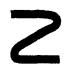
\includegraphics[keepaspectratio]{images/part001_ed0b989f.jpg}}

Moreover, if H is a Riesz space (fully lattice-ordered or not) it can happen that the supremum in H of two elements of H is different from their supremum in E (Exer. 3 b)). Finally, it can happen that H is fully lattice-ordered, that the supremum of each finite subset of H is the same in E and in H, but that there exist infinite subsets of H, bounded above in H, for which the suprema in E and H are different (Exer. 13 f)).

Let \((\mathrm{E}_{\iota})_{\iota \in \mathrm{I}}\) be any family of ordered vector spaces. Recall that, in the product space \(\mathrm{E} = \prod_{\iota \in \mathrm{I}}\mathrm{E}_{\iota}\) , the product order relation of the order relations of the factor spaces is the relation \(\ll x_{\iota}\leqslant y_{\iota}\) for all \(\iota \in \mathrm{I}\gg (\mathrm{S},\mathrm{III},\S 1,\mathrm{No.~4})\) . One verifies immediately that this relation is compatible with the vector space structure of E; E, equipped with this structure, is called the product space of the ordered spaces \(E_{\iota}\) .

PROPOSITION 3. --- Let \((\mathbf{E}_{\iota})_{\iota\in\mathbb{I}}\) be a family of ordered vector spaces. For the product space \(E=\prod_{\iota\in I}E_{\iota}\) to be a Riesz space (resp. a fully lattice-ordered space), it is necessary and sufficient that each of the spaces \(E_{\iota}\) be a Riesz space (resp. a fully lattice-ordered space).

Let us restrict ourselves to examining the case of fully lattice-ordered spaces. Suppose that all of the \(E_{\iota}\) are fully lattice-ordered; let A be a nonempty subset of E that is bounded above and let \(a = (a_{\iota})\) be an upper bound for A. For every \(\iota \in I\) , \(pr_{\iota}A\) is bounded above by \(a_{\iota}\) , hence has a supremum \(b_{\iota}\) in \(E_{\iota}\) ; it is clear that \(b = (b_{\iota})\) is the supremum of A in E.

Conversely, suppose E is fully lattice-ordered. Let \(A_{\kappa}\) be a subset of \(E_{\kappa}\) that is bounded above, \(A_{\kappa}^{\prime}\) the subset of E formed by the \(x = (x_{\iota})\) such that \(x_{\kappa} \in A_{\kappa}\) and \(x_{\iota} = 0\) for \(\iota \neq \kappa\) . It is immediate that \(A_{\kappa}^{\prime}\) is bounded above in E, hence has a supremum \(b = (b_{\iota})\) ; by the definition of the product order relation, necessarily \(b_{\iota} = 0\) for \(\iota \neq \kappa\) , and \(b_{\kappa}\) is the supremum of \(A_{\kappa}\) , which completes the proof.

DEFINITION 3. --- Let E be an ordered vector space, V and W two supplementary linear subspaces of E. One says that E is the ordered direct sum of V and W if the canonical mapping \((x,y)\mapsto x+y\) of the ordered vector space \(V\times W\) onto the ordered vector space E is an isomorphism.

PROPOSITION 4. --- For an ordered vector space E to be the ordered direct sum of two supplementary linear subspaces V, W, it is necessary and sufficient that the relations \(x \in V\) , \(y \in W\) , \(x + y \geqslant 0\) imply \(x \geqslant 0\) and \(y \geqslant 0\) .

Since \(x \geqslant 0\) and \(y \geqslant 0\) imply \(x + y \geqslant 0\) in E, the condition in the statement says that \((x, y) \mapsto x + y\) transforms the set of elements \(\geqslant 0\) of \(V \times W\) into the set of elements \(\geqslant 0\) of E.

\subsection{Bands in a fully lattice-ordered space}

DEFINITION 4. --- In a fully lattice-ordered space E, a linear subspace B of E is said to be a band if it satisfies the following conditions: 1) the relations \(x \in B\) , \(y \in E\) and \(|y| \leqslant |x|\) imply \(y \in B\) ; 2) for every nonempty subset X of B that is bounded above in E, the supremum sup X of X in E belongs to B.

Example. --- In the space \(R^{A}\) of real-valued functions defined on a set A, the set of functions that are zero at all the points of a subset M of A is a band.

\pandocbounded{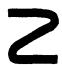
\includegraphics[keepaspectratio]{images/part001_20a85035.jpg}}

Remark. --- In the space \(R^{A}\) , the subspace \(\mathcal{B}(A)\) of bounded real-valued functions on A satisfies condition 1) of Def. 4; moreover, for every subset X of \(\mathcal{B}(A)\) that is bounded above in \(\mathcal{B}(A)\) , the upper envelope of X belongs to \(\mathcal{B}(A)\) . However, if A is infinite, a subset of \(\mathcal{B}(A)\) may be bounded above in \(R^{A}\) without being bounded above in \(\mathcal{B}(A)\) , in which case \(\mathcal{B}(A)\) is not a band in \(R^{A}\) .

It follows at once from Def. 4 that if B is a band in E then, for every nonempty subset X of B that is bounded below in E, inf X belongs to B. Every band B in E, equipped with the ordered vector space structure induced by that of E, is a fully lattice-ordered space and, for every subset \(X \subset B\) that is bounded above in B, the supremum of X in B is identical with its supremum in E.

The intersection of any family of bands in a fully lattice-ordered space E is also a band. For every subset \(M \subset E\) , there exists a smallest band containing M (since E itself is a band); this band will be called the band generated by M.

The properties of bands in a fully lattice-ordered space rest on the following proposition:

PROPOSITION 5. --- Let E be a fully lattice-ordered space, A a non-empty subset of E consisting of elements \(\geqslant 0\) , such that: 1) \(A + A \subset A\) , and 2) the relations \(x \in A\) , \(0 \leqslant y \leqslant x\) imply \(y \in A\) . Let M be the set of suprema in E of those subsets of A that are bounded above in E. Under these conditions, every element \(x \geqslant 0\) of E may be written in the form \(y + z\) , where \(y \in M\) is the supremum of the elements \(v \in A\) such that \(v \leqslant x\) , and where z is an element \(\geqslant 0\) that is alien to every element of M.

At any rate \(y \leqslant x\) , so it all comes down to showing that z = x - y is alien to every element \(t \in A\) (No.~1), in other words that \(u = \inf(z, t)\) is zero. By hypothesis, \(u \in A\) and \(u \leqslant x - y\) , thus \(u + y \leqslant x\) ; for every \(v \in A\) such that \(v \leqslant x\) , by definition \(v \leqslant y\) , thus \(u + v \leqslant u + y \leqslant x\) ; since \(u + v \in A\) by hypothesis, also \(u + v \leqslant y\) by the definition of y; finally, since \(u + y\) is the supremum in E of the elements \(u + v\) such that \(v \in A\) and \(v \leqslant x\) , we have \(u + y \leqslant y\) , whence \(u \leqslant 0\) , which completes the proof.

THEOREM 1 (F. Riesz). --- Let A be a subset of a fully lattice-ordered space E. The set A' of elements that are alien to every element of A is a band; the band A'\,' of elements that are alien to every element of A' is identical to the band generated by A, and E is the ordered direct sum of the bands A' and A'\,'.

The properties of alien elements, reviewed in No.~1, and the definition of a band, show at once that A' is a band, hence so is A'\,'. By Proposition 5 and the definition of a band, every element \(x \geqslant 0\) of E may be written \(x = y + z\) , with \(y \in A'\) and \(z \in A''\) , y and z being \(\geqslant 0\) ; since every element of E is the difference of two elements \(\geqslant 0\) , we have \(E = A' + A''\) ; on the other hand, since 0 is the only element alien to itself, we have \(A' \cap A'' = \{0\}\) , which proves that E is the direct sum of \(A'\) and \(A''\) ; finally, since the components in \(A'\) and \(A''\) of an element \(\geqslant 0\) of E are \(\geqslant 0\) , E is the ordered direct sum of \(A'\) and \(A''\) (No.~4, Prop. 4).

It remains to show that \(A''\) is identical to the band B generated by A. Now, E is the direct sum of B and the band \(B'\) formed by the elements alien to all the elements of B; since \(A \subset B\) , we have \(B' \subset A'\) ; on the other hand \(B \subset A''\) and E is also the direct sum of \(A'\) and \(A''\) ; therefore necessarily \(B = A''\) , \(B' = A'\) .

Theorem 1 and Proposition 5 make it possible to give another definition of the band generated by a set of elements of E:

PROPOSITION 6. --- Let E be a fully lattice-ordered space, M a subset of E, and B the band generated by M. Let \(M_{1}\) be the set of elements \(\geqslant 0\) of E each of which is \(\leqslant\) some element of the form \(\sum |x_{i}|\) , where \(x_{i} \in M\) ;

let \(M_{2}\) be the set of suprema of those subsets of \(M_{1}\) that are bounded above; then the set \(M_{2}\) is identical with the set of elements \(\geqslant0\) of B.

Clearly \(M_{2} \subset B\) by the definition of a band; on the other hand, if \(B'\) is the band of elements that are alien to every element of \(M_{1}\) , Theorem 1 shows that E is the ordered direct sum of B and \(B'\) . But Proposition 5 shows that every element \(\geqslant 0\) of E is the sum of an element of \(M_{2}\) and an element of \(B'\) , whence the proposition.

COROLLARY. --- Let \(a\) be an element of a fully lattice-ordered space \(\mathbf{E}\) , \(\mathbf{B}_a\) the band generated by \(a\) , \(\mathbf{B}_a'\) the band of elements alien to \(a\) . For every element \(x \geqslant 0\) of \(\mathbf{E}\) , the component of \(x\) in \(\mathbf{B}_a\) (for the decomposition of \(\mathbf{E}\) as the ordered direct sum of \(\mathbf{B}_a\) and \(\mathbf{B}_a'\) ) is equal to \(\sup_{n \in \mathbf{N}} \left( \inf(n|a|, x) \right)\) .

This follows from Proposition 6, applied to \(\mathbf{M} = \{a\}\) , and Proposition 5.

Note that the bands generated by a and \(|a|\) are identical. If a and b are two elements of E that are alien to each other, and if A and B are the bands generated by a and b, respectively, then every element of A is alien to every element of B; for, b belongs to the band \(A'\) of elements alien to a, whence \(B \subset A'\) , and, by Theorem 1, every element of A is alien to every element of \(A'\) .

\section{LINEAR FORMS ON A RIESZ SPACE}

\subsection{Positive linear forms on a Riesz space}

We recall the following definition (TVS, II, §2, No.~5):

DEFINITION 1. --- Given an ordered vector space E, a linear form L on E is said to be positive if \(L(x) \geqslant 0\) for every \(x \geqslant 0\) in E.

Since \(L(y) - L(x) = L(y - x)\) , it is the same to say that the relation \(x \leqslant y\) implies \(L(x) \leqslant L(y)\) , or again that \(L\) is an increasing function on \(\mathbf{E}\) .

Examples. --- 1) Let A be any set, E a linear subspace of the space \(R^{A}\) of all real-valued functions defined on A. For every element \(a \in A\) , the mapping \(x \mapsto x(a)\) is a positive linear form on E.

\begin{enumerate}
\def\labelenumi{\arabic{enumi})}
\setcounter{enumi}{1}
\item
  Let \(\mathrm{I} = [a, b]\) be a compact interval of \(\mathbf{R}\) , \(\mathrm{E}\) the Riesz space formed by the regulated real-valued functions on \(\mathrm{I}\) (FRV, II, §1, No.~3); the mapping \(x \mapsto \int_{a}^{b} x(t) dt\) is a positive linear form on \(\mathrm{E}\) .
\item
  Let F be any set, U an ultrafilter on F (GT, I, §6, No.~4), E the Riesz space \(\mathcal{B}(F)\) of bounded real-valued functions on F. For every \(x \in E\) , \(\lim_{\mathfrak{U}} x(t)\) exists, because \(x(\mathfrak{U})\) is a base of an ultrafilter on the relatively compact set \(x(F)\) , hence is convergent. Moreover, if \(x \geqslant 0\) then \(\lim_{\mathfrak{U}} x(t) \geqslant 0\) by the principle of extension of inequalities; the mapping \(x \mapsto \lim_{\mathfrak{U}} x\) is thus a positive linear form on E. If U is taken to be the ultrafilter formed by the sets containing an element \(a \in F\) , one recovers the positive linear form \(x \mapsto x(a)\) (Example 1).
\end{enumerate}

PROPOSITION 1. --- Let E be an ordered vector space, L a mapping of E into R such that \(L(x+y)=L(x)+L(y)\) and such that the relation \(x\geqslant0\) implies \(L(x)\geqslant0\) ; then \(L(\lambda x)=\lambda L(x)\) for every scalar \(\lambda\) and every \(x\geqslant0\) .

Since \(L(-x) = -L(x)\) (L being a representation of the additive group E in R), we can restrict ourselves to the case that \(\lambda \geqslant 0\) . For every integer \(n \geqslant 0\) , we have \(L(nx) = nL(x)\) , whence \(L((1/n)x) = (1/n)L(x)\) and consequently \(L(rx) = rL(x)\) for every rational number \(r \geqslant 0\) . On the other hand, L is increasing in E; if r and \(r'\) are rational numbers such that \(r \leqslant \lambda \leqslant r'\) , it follows that \(rL(x) \leqslant L(\lambda x) \leqslant r'L(x)\) ; since \(rL(x)\) and \(r'L(x)\) differ from \(\lambda L(x)\) as little as we like, we have \(L(\lambda x) = \lambda L(x)\) .

PROPOSITION 2. --- Let E be a real vector space, C a convex cone with vertex 0 in E such that E = C - C, and \(x \mapsto M(x)\) a mapping of C into R such that \(M(\lambda x + \mu y) = \lambda M(x) + \mu M(y)\) for all \(x \in C\) , \(y \in C\) , \(\lambda \geqslant 0\) , \(\mu \geqslant 0\) . Then, there exists one and only one linear form L that extends M to E.

By hypothesis, every \(z \in E\) may be written \(z = y - x\) , where x, y belong to C; moreover, if also \(z = y' - x'\) with \(x' \in C\) , \(y' \in C\) , then

\(M(y) - M(x) = M(y') - M(x')\) ; for, from the relation \(y - x = y' - x'\) we infer \(y + x' = x + y'\) , consequently \(M(y) + M(x') = M(x) + M(y')\) . Let us denote by \(L(z)\) the common value of \(M(y) - M(x)\) for all expressions of \(z\) as the difference \(y - x\) of two elements of C; one verifies immediately that \(L\) is a linear form on E extending \(M\) ; the uniqueness of \(L\) results from the fact that C generates the space E.

PROPOSITION 3. --- Let E be a directed ordered vector space, P the set of elements \(\geqslant 0\) of E, and \(x \mapsto M(x)\) a mapping of P into R, with values \(\geqslant 0\) , such that \(M(x + y) = M(x) + M(y)\) for all x, y in P. Then, there exists one and only one positive linear form L that extends M to E.

Since E = P - P, the same reasoning as in Prop. 2 proves, first, the existence and uniqueness of an additive mapping L of E into R that extends M. Proposition 1 then shows that \(L(\lambda x) = \lambda L(x)\) for all \(\lambda \geqslant 0\) and all \(x \in P\) , from which it is immediate that L is a linear form.

\subsection{Relatively bounded linear forms}

Let E be a directed ordered vector space. Let Q be the set of positive linear forms on E; it is a subset of the algebraic dual \(E^{*}\) of E (the space of all linear forms on E). It is immediate that \(Q + Q \subset Q\) and \(\lambda Q \subset Q\) for every scalar \(\lambda > 0\) (in other words, Q is a convex cone in \(E^{*}\) ). Moreover, \(Q \cap (-Q) = \{0\}\) , because if L and -L are both positive linear forms, then \(L(x) \geqslant 0\) and \(L(x) \leqslant 0\) for all \(x \geqslant 0\) , whence \(L(x) = 0\) for all \(x \geqslant 0\) and therefore L = 0 (No.~1, Prop. 3). The set Q thus defines on \(E^{*}\) an order relation \(L \leqslant M\) , equivalent to «M - L is a positive linear form on E», or again to «for every \(x \geqslant 0\) , \(L(x) \leqslant M(x)\) »; the elements \(\geqslant 0\) of \(E^{*}\) for this order structure are the positive linear forms (which justifies the terminology introduced). Let \(\Omega\) be the linear subspace of \(E^{*}\) generated by Q, that is, the set of linear forms on E that are differences of two positive linear forms; we are going to give another characterization of the elements of \(\Omega\) when E is a Riesz space.

DEFINITION 2. --- Given a Riesz space E, a linear form L on E is said to be relatively bounded if, for every \(x \geqslant 0\) in E, L is bounded on the set of \(y \in E\) such that \(|y| \leqslant x\) .

THEOREM 1. --- \(1^{\circ}\) In order that a linear form L on a Riesz space E be relatively bounded, it is necessary and sufficient that it be the difference of two positive linear forms.

\(2^{\circ}\) The ordered vector space \(\Omega\) of relatively bounded linear forms on E is a Riesz space that is fully lattice-ordered.

If \(L = U - V\) , where \(U\) and \(V\) are positive linear forms on \(\mathbf{E}\) , the relation \(-x \leqslant y \leqslant x\) implies

\[
- U (x) \leqslant U (y) \leqslant U (x) \quad \text { and } \quad - V (x) \leqslant V (y) \leqslant V (x),
\]

whence it is immediate that \(|L(y)| \leqslant U(x) + V(x)\) ; thus, L is relatively bounded. Suppose, conversely, that L is relatively bounded; it all comes down to proving that there exists a positive linear form N such that \(N(x) \geqslant L(x)\) for all \(x \geqslant 0\) , because N - L will then be a positive linear form.

Now, if a positive linear form N has this property then, for every \(x \geqslant 0\) and for \(0 \leqslant y \leqslant x\) , we have \(N(x) \geqslant N(y) \geqslant L(y)\) , therefore \(N(x) \geqslant \sup_{0 \leqslant y \leqslant x} L(y)\) ; if we prove that the real-valued function

\[
x \mapsto M (x) = \sup _ {0 \leqslant y \leqslant x} L (y),
\]

defined on the set P of elements \(\geqslant0\) of E, may be extended to a positive linear form on E (to be denoted M as well), we will have demonstrated the first part of the theorem and will have proved, moreover, that M is the supremum of 0 and L in \(\Omega\) . Since \(M(x)\geqslant0\) on P, it all comes down to proving that

\[
M (x + x ^ {\prime}) = M (x) + M (x ^ {\prime})
\]

for every pair of elements \(x \geqslant 0\) , \(x' \geqslant 0\) of E (No.~1, Prop. 3). By definition,

\[
\begin{array}{c} M (x) + M (x ^ {\prime}) = \sup _ {0 \leqslant y \leqslant x} L (y) + \sup _ {0 \leqslant y ^ {\prime} \leqslant x ^ {\prime}} L (y ^ {\prime}) \\ = \sup _ {0 \leqslant y \leqslant x, 0 \leqslant y ^ {\prime} \leqslant x ^ {\prime}} L (y + y ^ {\prime}) \leqslant M (x + x ^ {\prime}). \end{array}
\]

On the other hand, for every \(z\) such that \(0 \leqslant z \leqslant x + x'\) , we have \(x + x' = z + u\) with \(u \geqslant 0\) ; by the decomposition lemma (§1, No.~1), there exist two elements \(y, y'\) such that \(0 \leqslant y \leqslant x\) , \(0 \leqslant y' \leqslant x'\) and such that \(z = y + y'\) , \(u = (x - y) + (x' - y')\) ; then

\[
L (z) = L (y) + L \left(y ^ {\prime}\right) \leqslant M (x) + M \left(x ^ {\prime}\right),
\]

therefore \(M(x + x') = \sup_{0 \leqslant z \leqslant x + x'} L(z) \leqslant M(x) + M(x')\) , which completes the proof of the first part of the theorem. Moreover, we have thus shown that \(\Omega\) is a Riesz space and that, for every relatively bounded linear form L on E and for every \(x \geqslant 0\) ,

\[
L ^ {+} (x) = \sup _ {0 \leqslant y \leqslant x} L (y).\tag{1}
\]

It remains to see that \(\Omega\) is fully lattice-ordered; for this, it suffices to show that any set H of positive linear forms, bounded above and directed for the relation \(\leqslant\) , has a supremum in \(\Omega\) .

More generally, we have the following lemma:

Lemma. --- Let E be a directed ordered vector space, \(E^{*}\) its dual, ordered by taking as positive elements the positive linear forms. Let \((u_{\alpha})\) be an increasing directed family of elements of \(E^{*}\) . If, for every \(x \geqslant 0\) in E, \(\sup u_{\alpha}(x) < +\infty\) , then the family \((u_{\alpha})\) has a supremum u in \(E^{*}\) and, for all \(x \geqslant 0\) in E,

\[
u (x) = \sup _ {\alpha} u _ {\alpha} (x).\tag{2}
\]

In the set P of all \(x \geqslant 0\) in E, define the mapping u by the formula (2); it is immediate that \(u(\lambda x) = \lambda u(x)\) for all \(\lambda \geqslant 0\) and \(x \in P\) ; to prove the lemma it therefore suffices, by Prop. 2 of No.~1, to show that

\[
u (x + y) = u (x) + u (y)
\]

for \(x, y\) in P. But this is immediate on observing that \(u(x) = \lim u_{\alpha}(x)\) with respect to the directed set of indices (monotone limit theorem).

From the formula (1), one deduces immediately that if L and M are two relatively bounded linear forms on E then, for every \(x \geqslant 0\) ,

\[
\left\{ \begin{array}{l} \sup (L, M) (x) = \sup _ {y \geqslant 0,   z \geqslant 0,   y + z = x} \big (L (y) + M (z) \big) \\ \inf (L, M) (x) = \inf _ {y \geqslant 0,   z \geqslant 0,   y + z = x} \big (L (y) + M (z) \big). \end{array} \right.\tag{3}
\]

In particular if, in the first of these formulas, \(M\) is replaced by \(-L\) , we get

\[
| L | (x) = \sup _ {y \geqslant 0, z \geqslant 0, y + z = x} L (y - z).
\]

Now, if \(x = y + z\) , \(y \geqslant 0\) and \(z \geqslant 0\) , then \(-x \leqslant y - z \leqslant x\) ; conversely, the relation \(|u| \leqslant x\) implies \(L(u) \leqslant |L|(|u|) \leqslant |L|(x)\) . From this we deduce the formula

\[
| L | (x) = \sup _ {| y | \leqslant x} L (y) \quad \text { for } x \geqslant 0,\tag{4}
\]

whence, in particular,

\[
| L (x) | \leqslant | L | (| x |)\tag{5}
\]

for all \(x \in \mathbf{E}\) .

PROPOSITION 4. --- In order that two positive linear forms L, M on a Riesz space E be alien to each other in the space \(\Omega\) , it is necessary and sufficient that, for every number \(\varepsilon > 0\) and every \(x \geqslant 0\) in E, there exist two elements \(y \geqslant 0\) , \(z \geqslant 0\) of E such that \(x = y + z\) and \(L(y) + M(z) \leqslant \varepsilon\) . Indeed, by the second formula of (3), this condition expresses that \(\inf(L, M) = 0\) .

PROPOSITION 5. --- Let L be a positive linear form on a Riesz space E. In order that a positive linear form M on E belong to the band generated by L in \(\Omega\) , it is necessary and sufficient that, for every \(x \geqslant 0\) in E and every number \(\varepsilon > 0\) , there exist a number \(\delta > 0\) such that the relations \(0 \leqslant y \leqslant x\) and \(L(y) \leqslant \delta\) imply \(M(y) \leqslant \varepsilon\) .

Let us first show that the condition is necessary. If \(M \geqslant 0\) belongs to the band generated by L in \(\Omega\) , then (§1, No.~5, Cor. of Prop. 6)

\[
M = \sup _ {n} \left(\inf (n L, M)\right).
\]

If one sets

\[
U _ {n} = M - \inf (n L, M),
\]

\(U_{n}\) is thus a positive linear form on E and \(\inf_{n} U_{n} = 0\) in \(\Omega\) ; consequently (Lemma) \(U_{n}(x)\) tends to 0 as n tends to infinity, and there exists an n such that \(U_{n}(x) \leqslant \varepsilon / 2\) . Fixing such an n, we have \(U_{n}(y) \leqslant \varepsilon / 2\) for all y such that \(0 \leqslant y \leqslant x\) , thus the relation \(0 \leqslant y \leqslant x\) implies

\[
M (y) \leqslant \frac {\varepsilon}{2} + \inf (n L, M) (y) \leqslant \frac {\varepsilon}{2} + n L (y);
\]

if \(y\) is such that \(L(y) \leqslant \varepsilon / 2n\) it follows that \(M(y) \leqslant \varepsilon\) , which establishes our assertion.

Let us now show that the condition is sufficient. For every positive linear form \(M\) on \(\mathrm{E}\) , one can write \(M = U + V\) , where \(U\) belongs to the band generated by \(L\) in \(\Omega\) and where \(V\) is alien to \(L\) , \(U\) and \(V\) being positive (§1, No.~5, Th. 1). If \(M\) satisfies the condition of the statement then so does \(V = M - U\) , since \(0 \leqslant V \leqslant M\) . From this we will deduce that \(V = 0\) . For every \(x \geqslant 0\) in \(\mathrm{E}\) and every number \(\eta > 0\) , there exist two elements \(y \geqslant 0\) , \(z \geqslant 0\) of \(\mathrm{E}\) such that \(x = y + z\) and \(L(y) + V(z) \leqslant \eta\) (Prop. 4); given an arbitrary number \(\varepsilon > 0\) , choose \(\eta \leqslant \varepsilon\) so that the relations \(0 \leqslant u \leqslant x\) and \(L(u) \leqslant \eta\) imply \(V(u) \leqslant \varepsilon\) ; with \(y\) and \(z\) then determined as above, we have \(L(y) \leqslant \eta\) , therefore \(V(y) \leqslant \varepsilon\) and so

\[
V (x) = V (y) + V (z) \leqslant \varepsilon + \eta \leqslant 2 \varepsilon ;
\]

since \(\varepsilon\) is arbitrary, we have \(V(x) = 0\) for every \(x \geqslant 0\) , that is, \(V = 0\) .

Example. --- Let E be a Riesz space equipped with a locally convex topology compatible with its ordered vector space structure (TVS, II, §2, No.~7). Let \(E'\) be the topological dual of E, and suppose in addition that the cone P of elements \(\geqslant 0\) of E is complete for the weakened topology \(\sigma(\mathrm{E},\mathrm{E}')\) . Then every continuous linear form \(x' \in E'\) is relatively bounded, for one knows (TVS, II, §6, No.~8, Cor. 2 of Prop. 11) that under these conditions, for every \(x \geqslant 0\) in E the set of \(y \in E\) such that \(|y| \leqslant x\) is compact for \(\sigma(\mathrm{E},\mathrm{E}')\) . From this we deduce that E is then fully lattice-ordered; for (§1, No.~3, Prop. 2), it suffices to show that for every set \(H \subset E\) that is bounded above and directed for \(\leqslant\) , the section filter F of H is convergent in E for the topology \(\sigma(\mathrm{E},\mathrm{E}')\) (the latter being compatible with the ordered vector space structure of E). By translation, we can suppose that \(H \subset P\) , and it then suffices to show that F is a Cauchy filter for \(\sigma(\mathrm{E},\mathrm{E}')\) , or again that every continuous linear form \(x' \in E'\) has a limit with respect to F. But this follows at once from the monotone limit theorem when \(x'\) is a positive linear form, and since every linear form \(x' \in E'\) is the difference of two positive linear forms (Th. 1) our assertion is proved.
